%--------------------------------------------------------------------------------


\documentclass[12pt]{article}
\usepackage[T1]{fontenc}
\usepackage[bf]{caption}
\usepackage{hyperref}
\usepackage[all]{hypcap}
\usepackage[utf8]{inputenc}
\usepackage{graphicx}
\usepackage[english]{babel}
\selectlanguage{english}
\usepackage{subfig}                % \subfloat
\usepackage{color}
\usepackage{url}
\inputencoding{utf8}
%\usepackage[bf]{caption2}
\usepackage{hyperref}
\usepackage[all]{hypcap}
\hypersetup{colorlinks=false, linkbordercolor=1 1 1, citebordercolor=1 1 1}
\usepackage[right]{lineno}
\renewcommand\linenumberfont{\normalfont\tiny\color{blue}}


\title{Computer Vision Course}
\subtitle{Brno - University of technology}
\author{Emanuele Corongiu <xcoron02@stud.fit.vutbr.cz>}
\date{\today}


%--------------------------------------------------------------------------------


\begin{document}
\selectlanguage{english}
\maketitle

\section{Abstract}


%%%%%%%%%%%%%%%%%%%%%%%%%%%%%%%%%%%%%%%%%%%%%%%%%%%%%%%%%%%%%%%%%%%%%%%%%%%%%%%%%%%%%%%%

\section{Yolo V8}



\begin{equation}
  \label{moje-rovnice}
  c = a + b
\end{equation}

sdfsdfsdfsdf \ref{fig:obrazek} sdfsdfsdfsdf

\begin{figure}[htb]
  \centering
  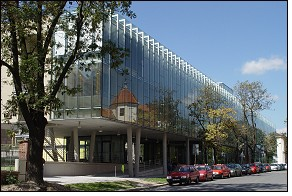
\includegraphics[width=5cm,keepaspectratio]{obrazek.jpg}
  \caption{try \cite{wikipedia}}
  \label{fig:try}
\end{figure}


%%%%%%%%%%%%%%%%%%%%%%%%%%%%%%%%%%%%%%%%%%%%%%%%%%%%%%%%%%%%%%%%%%%%%%%%%%%%%%%%%%%%%%%%



\bibliographystyle{alpha}
\begin{flushleft}
  \bibliography{project}
\end{flushleft}

%\appendix
%\newpage
%\section{}

\end{document}
